\documentclass[10pt]{article}

\usepackage{titlesec}

% Section titles and subsection titles settings
\titleformat{\section}{\normalfont\large\bfseries}{\thesection}{2em}{}
\titlespacing*{\section}{2pt}{*1}{*1}
\titleformat{\subsection}{\normalfont\small\bfseries}{\thesubsection}{1em}{}[]
\titlespacing{\subsection}{0pt}{0.6\baselineskip}{0.6\baselineskip}

% Font
\usepackage{fontspec}
\setmainfont{Arial}

% Page layout
\usepackage[a4paper,margin=0.75in]{geometry}

% Math
\usepackage{mathptmx}  

% Fonts
\usepackage{fontspec}

% Hyperlinks
\usepackage{hyperref}

% Colors
\usepackage{xcolor}

% Tables
\usepackage{booktabs}
\usepackage{siunitx}

% Figures
\usepackage{graphicx}
\usepackage{caption}
\captionsetup[figure]{skip=2pt} 



% Title and Author information
\title{
    \vspace{-2cm}Classification Model Generalization on NinaPro Dataset
}
\author{
    \vspace{0.2cm}Antea Ceko, Chiara Billi, Irene Vardabasso, Ludek Cizinsky, Lou Houngbedji \\
    \vspace{0.2cm} \normalsize{Ecole Polytechnique Fédérale de Lausanne, Switzerland}
}

\date{\today}

\begin{document}
\maketitle

\section{Introduction}
In recent years, Machine Learning based approaches have seen success in many fields, including the medical field.
In this project, we aim to assess various classification models that can predict the type of movement performed by a patient based on the EMG signals recorded from the patient's forearm.
The dataset used for this project is the NinaPro dataset DB1 \cite{ninapro}, which contains EMG signals recorded from 27 patients performing different hand movements. 

\section{Dataset and Preprocessing Steps}
\subsection{General Information}
The surface electromyography (sEMG) data were captured with 10 electrodes, comprising 10 repetitions of 52 distinct movements. 
Participants viewed video prompts on a laptop screen and replicated the movements. Each repetition took 5 seconds, followed by a 3-second rest \cite{ninapro}.
The experiment encompassed three exercise categories: \textbf{1)} fundamental finger movements, \textbf{2)} isometric and isotonic hand configurations, along with basic wrist motions, and \textbf{3)} grasping and functional movements.
% TODO: possibly add the table about the participants


\subsection{Preprocessing}
For the purposes of our work, we decided to focus on the first category of movements, which includes 12 different movements and in total consists of $7.58$ hours of EMG signal data. 
Importantly, the alignment between the EMG signals and corresponding labels has already been done by the authors of the NinaPro dataset. Further, in addressing discrepancies between subject movements and software stimuli, 
the authors applied a generalized likelihood ratio algorithm to correct erroneous movement labels \cite{ninapro}. 
Importantly, the EMG signals were already preprocessed by the manufacturer of the electrodes,
using a Root Mean Square (RMS) filter. This motivated our choice to apply low-pass filtering to the sEMG signals at a cutoff frequency of $5 Hz$ using a zero-phase second-order Butterworth filter
similarly as Atzori et al \cite{ninapro}. 

% Include the preprocessing figure
\begin{figure}[h]
    \centering
    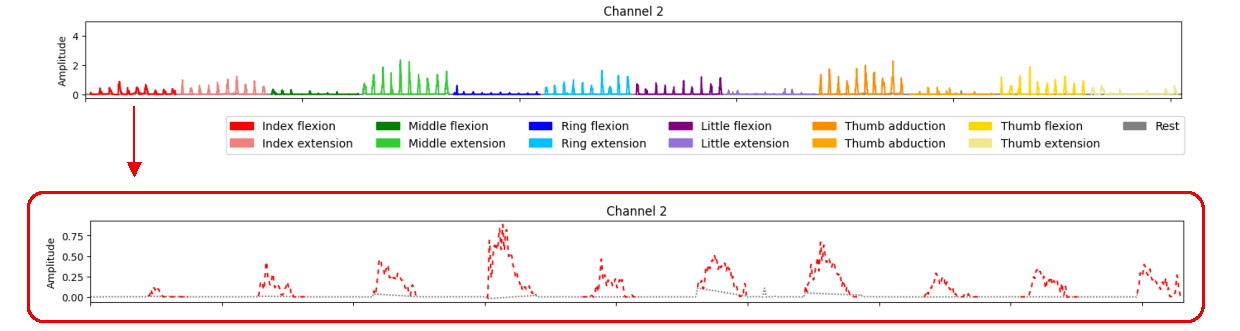
\includegraphics[width=1\textwidth]{../figures/preprocessing.pdf}
    \caption{First plot shows preprocessed EMG signal for the first subject for one of the 10 channels. The subsequent plot facilitates a closer look 
    at the \texttt{Index flexion} finger movement and the 10 repetitions. }
    \label{fig:preprocessing}
\end{figure}

\subsection{Data splitingg}
As the \ref{fig:preprocessing} shows, the EMG signals are recorded in 10 repetitions. Importantly,
there is a variation in amplitude of the EMG signals across the repetitions. Therefore, when spliting the data into training, validation and test sets, 
we made sure that each split is assigned with repetition from both the start and the end of the trial. Specifically,
we assigned the train split to the 1st, 3rd, 5th, 7th and 9th repetitions, the validation split to the 2nd, 4th and 8th repetitions, and the test split to the 6th and 10th repetitions.
This way, we ensured the model is trained and evaluated on the representative data. Notably, since each repetition of a given stimuli is associated with the rest period,
we assigned the rest period to the same split as the corresponding repetition.

Next, for each split and subject, we perfomed windowing with a window size of $500$ ms and a stride of $100$ ms. The chosen window size
allows to capture enough information about the movement to be able to classify it, while the chosen stride allows to capture the temporal dynamics of the movement and 
is a compromise between the computational cost and the amount of information captured. In addition, given data the sampling frequency of $100$ Hz, the chosen step size
means we get a sample for every time point. Importantly, the label for each window is assigned based on the majority label.

\begin{figure}[h]
    \centering
    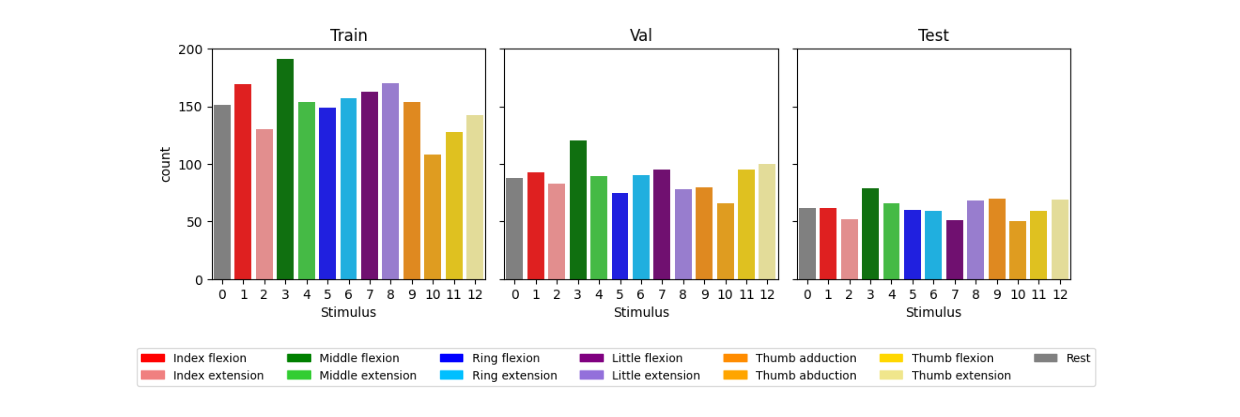
\includegraphics[width=1\textwidth]{../figures/downsampling.pdf}
    \caption{Distribution of the stimuli classes accross splits for the 17th subject.}
    \label{fig:downsampling}
\end{figure}

This windowing approach results in a significant class imbalance between stimuli classes (in total 40 \%) and the rest period (in total 60 \%).
Therefore, we decided to downsample the rest period to the average number of samples per class. This way, we ensured that the model is not biased towards the rest period.

\subsection{Feature Extraction}
For each window, we decided to extract both time and frequency domain features. For time, we extracted 
Mean Absolute Value (\texttt{MAV}), Maximum Absolute Value (\texttt{MaxAV}), Wavelength (\texttt{WL}), Standard Deviation (\texttt{STD}), and Root Mean Square (\texttt{RMS}). 
Additional, in the frequency domain, we considered Mean Power, Total Power, Mean Frequency, Median Frequency, and Peak Frequency. 

\begin{figure}[h]
    \centering
    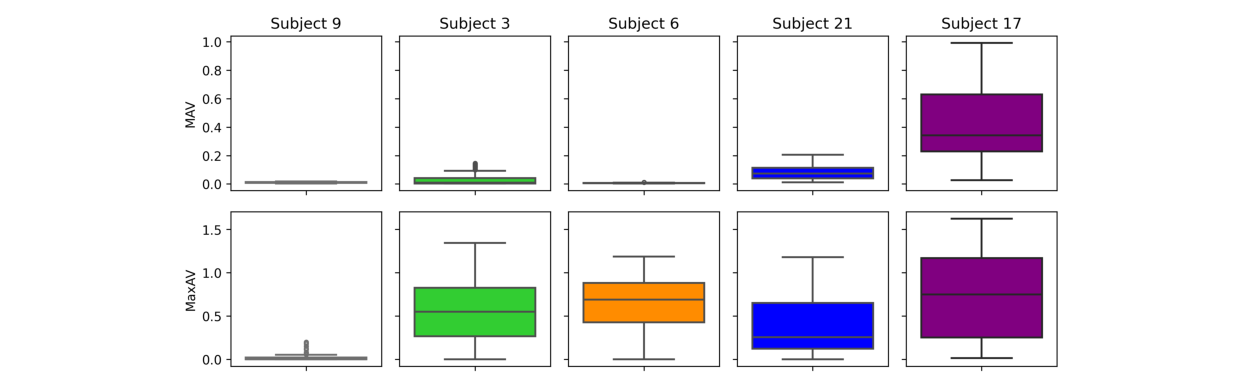
\includegraphics[width=1\textwidth]{../figures/inter_sub_var.pdf}
    \caption{Variability of selected features of Index Flexion stimuli, \texttt{MAV} and \texttt{MaxAV}, accross subjects. Boxplot showing median, 25th and 75th percentiles, and max-min of the features.}
    \label{fig:feat_var}
\end{figure}

% TODO: perhaps would be better if we gave more precise answer to why these difference occur
As the Figure \ref{fig:feat_var} shows, the extracted time features for the chosen stimuli significantly differ accross subjects.
These could be possibly explained via variations in physiological factors, such as muscle strength, anatomy, or motor control strategies. 
This is a known challenge when working with sEMG data which has been recently tackled in various works 
via deep learning based methods \cite{dl2, dl1}. 

% TODO: add standard scaling to the pipeline!
\section{Methods}
We start with training and evaluating chosen set of models on individual subjects. Namely, we use Logistic Regression (\texttt{LR}), K-Nearest Neighbors (\texttt{KNN})
and Random Forest (\texttt{RF}). We will conduct extensive grid search to find the optimal hyper-parameters for each model. 
This part of the experiment should confirm our base hypothesis that the chosen models are capable of generalising from given subject's training data to the corresponding validation data.
In addition, we will assess whether the models trained on individual subjects use similar features. In the second part of our experiment, we will choose the best performing model from the previous phase 
and train it on the selected  subset of subjects. Finally, we will evaluate its performance on data of subjects which were not seen during training phase.
We will vary the number of subjects in training dataset to observe the impact on the model's generalization capabilities.


\section{Results and Discussion}
\begin{table}[!h]
    \centering
    \begin{tabular}{llr}
        \toprule
        \textbf{Model} & \textbf{Best Configuration Accross Subjects} & \textbf{Test Acc $\pm$ 95CI} \\
        \midrule
        Random Forest & \texttt{MaxDepth=}15,\texttt{NofEstimators=}300, \texttt{MaxFeat=}\texttt{sqrt} & $\mathbf{0.82 \pm0.04}$ \\
        Softmax Regression & \texttt{Loss=hinge}, \texttt{Penalty=L1}, \texttt{Alpha=}=$1e^{-4}$, \texttt{MaxIter=}270 &  $0.74 \pm0.05$ \\
        K-Nearest Neighbors & \texttt{NofNeighbors=}2, \texttt{Weights=distance} &  $0.65 \pm0.05$ \\
        \bottomrule
    \end{tabular}
    \caption{Results of training and evaluating the chosen models on individual subjects. The best configuration for each model is a mean of the numeric hyper-parameters, and the most frequent value for the categorical hyper-parameters.}
    \label{tab:results1}
\end{table}

Table \ref{tab:results1} shows that the best performing model is by far \texttt{RF} which achieved 82 \%.
This is a comparable performance to the one reported by Atzori et al. \cite{ninapro},
however, our task for simplicity only consists of 12 movements instead of 52. Interestingly,
we were able to achieve solid performance even with the \texttt{SR} which is a linear model.
This suggests high quality of the extracted features making the prediction task easier for the model.
Last but not least, while it is important in general to consider 
regularisation, for our models, it played only a minor role (e.g. \texttt{SR}'s \texttt{Alpha} being only $1e^{-4}$), as the best configuration show.


\begin{figure}[h]
    \centering
    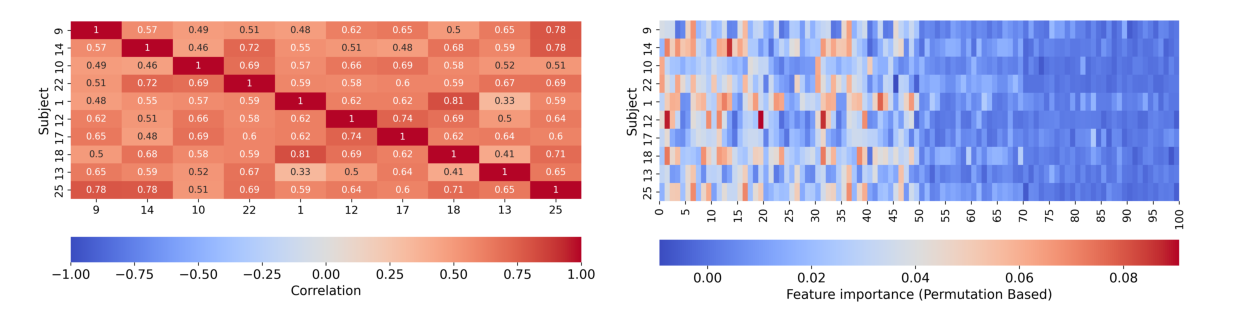
\includegraphics[width=1\textwidth]{../figures/fig_feat_imp.pdf}
    \caption{Both figures depict feature permutation importance for the \texttt{SF} 
    model. The left plot illustrates the correlation among individual subjects' feature 
    importance, while the right plot showcases the importance of each feature for every subject.}
    \label{fig:feat_imp}
\end{figure}

Figure \ref{fig:feat_imp} shows that the feature importance varies accross subjects. The left plot
suggests that there is relatively high correlation in how each subject ranks the features. However,
from the right plot, we can see that the high correlation could be likely explained by the 
last 50 features which are ranked very low by all subjects. In contrast, for the first 
50 features, there is a significant variation in the ranking. This is in line 
with the Figure \ref{fig:feat_var} that shows variability in the individual feature values
accross subjects, therefore, it is not surprising that the models trained on individual subjects
use different features.


\newpage
\bibliographystyle{abbrv}
\bibliography{references}

\end{document}